\documentclass[a4paper,12pt]{article}
\author{Grunda}
\usepackage[utf8]{inputenc}   
\usepackage[T2A]{fontenc}    
\usepackage[ukrainian]{babel} 
\usepackage{geometry}         
\usepackage{amsmath}          
\usepackage{amsfonts}         
\usepackage{amssymb}         
\usepackage{graphicx}         
\usepackage{hyperref}         
\usepackage{booktabs} 
\usepackage{caption}  
\usepackage{adjustbox} 
\usepackage{subcaption} 


\geometry{left=2.5cm, right=2.5cm, top=2.5cm, bottom=2.5cm}

\title{Звіт до лабораторної роботи №7}
\author{Ярослав Грунда \\ Фі-21, ФТІ КПІ}
\date{\today}

\begin{document}

\maketitle

\tableofcontents 
\newpage

\section{Мета роботи}
Реалiзацiя та порiвняльний аналiз модифiкацiй алгоритму швидкого сортування.
\section{Графіки повного порівняльного аналізу}
\begin{figure}[h!]
    \centering
    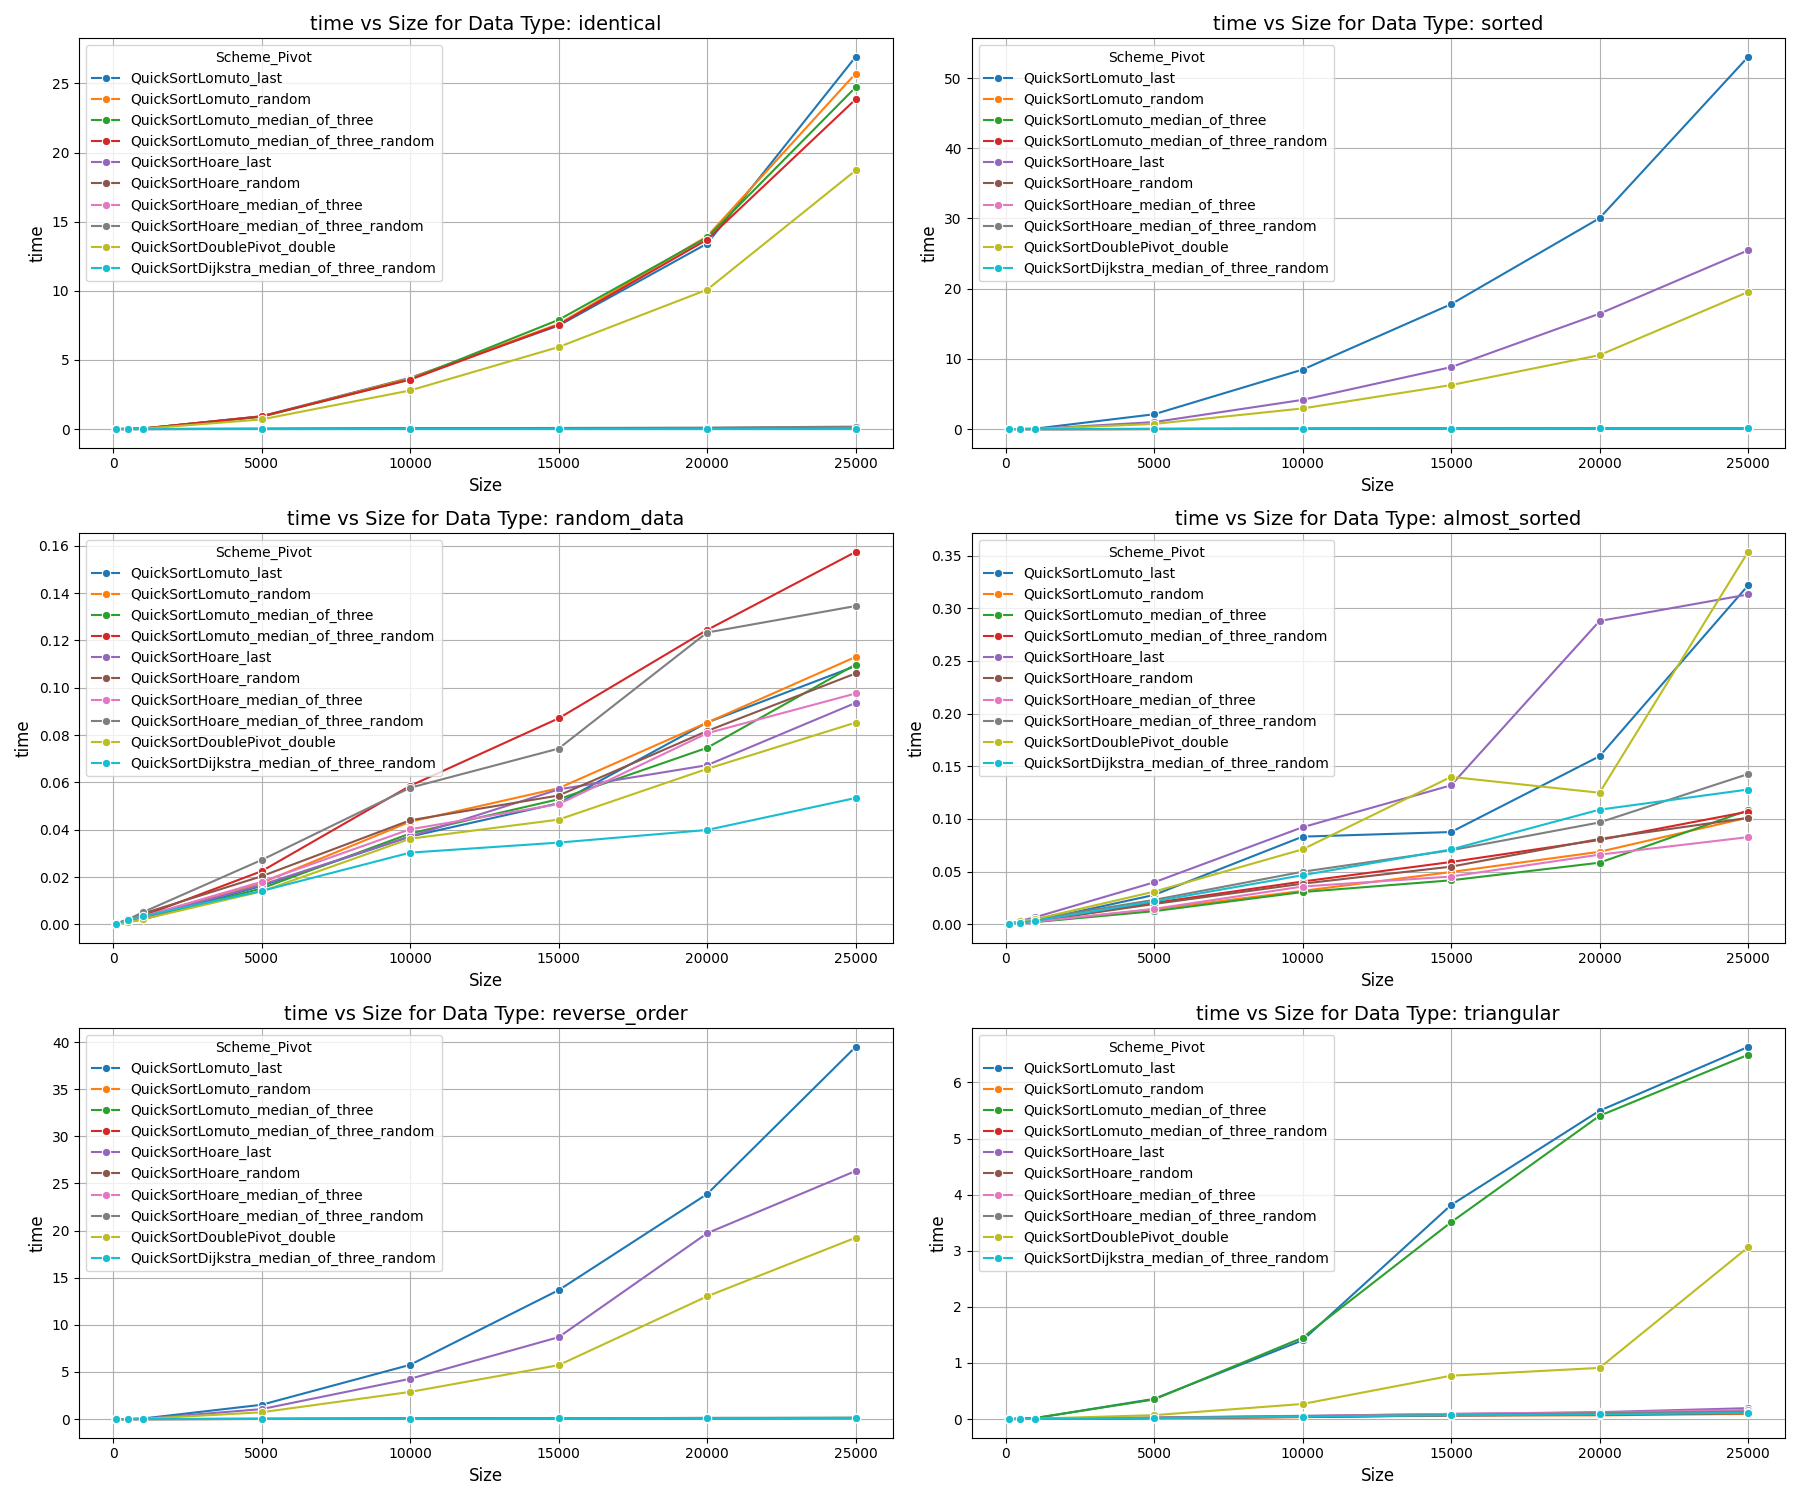
\includegraphics[width=\textwidth]{D://University/third_course/AppliedAlgorithms/lab7/time_plots/time_vs_size_all.png}
    \caption{Графік для часу.}
    \label{fig:time_chart}
\end{figure}
\newpage
\begin{figure}[h!]
    \centering
    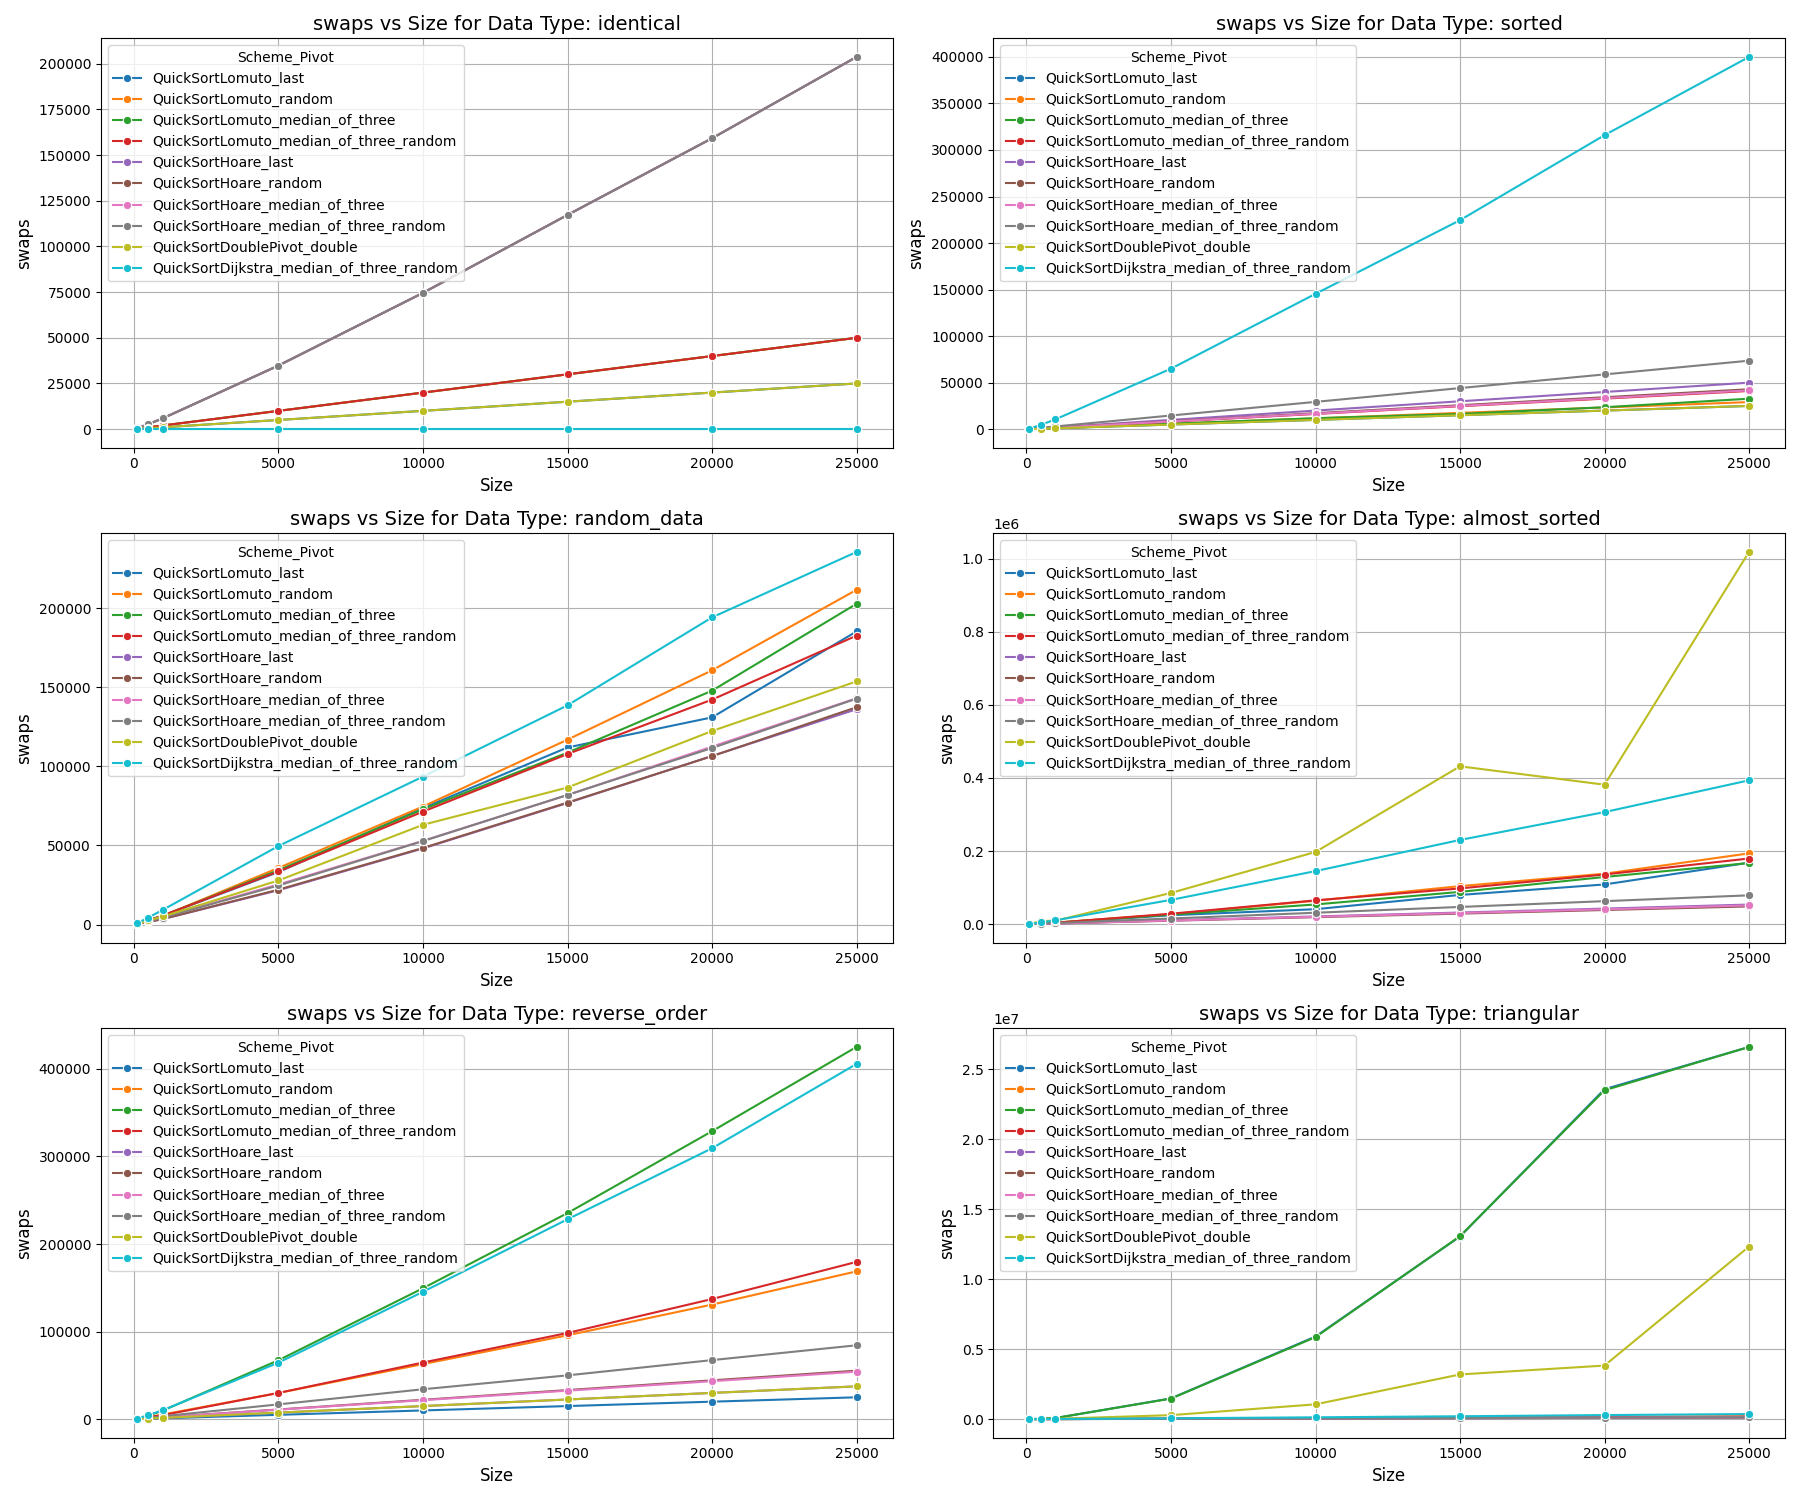
\includegraphics[width=\textwidth]{D://University/third_course/AppliedAlgorithms/lab7/swaps_plots/swaps_vs_size_all.png}
    \caption{Графік для переставлянь.}
    \label{fig:swaps_chart}
\end{figure}
\newpage
\begin{figure}[h!]
    \centering
    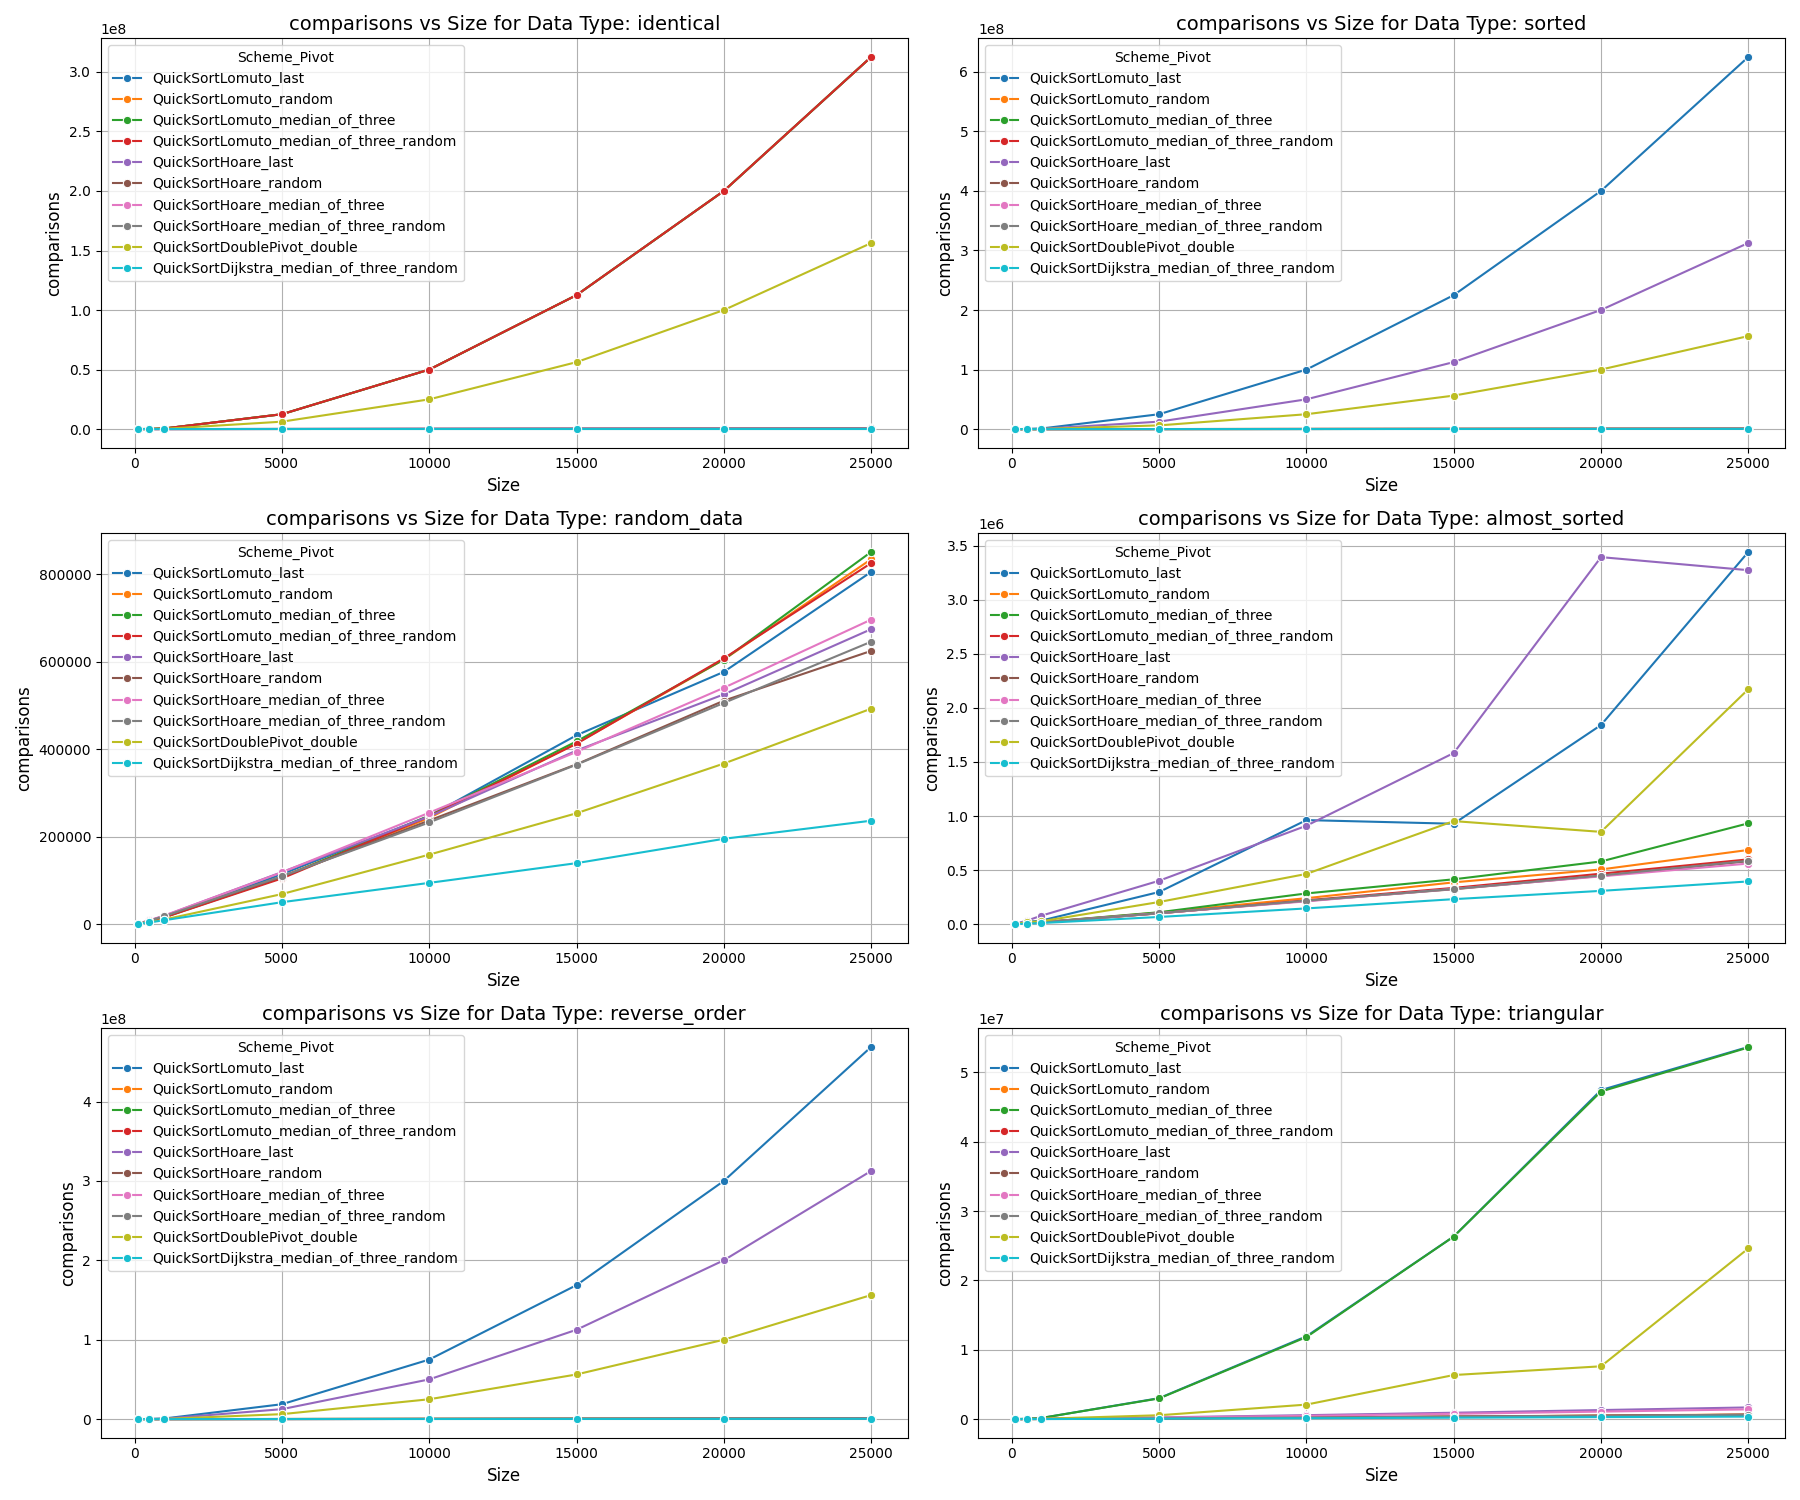
\includegraphics[width=\textwidth]{D://University/third_course/AppliedAlgorithms/lab7/comparisons_plots/comparisons_vs_size_all.png}
    \caption{Графік для порівнянь.}
    \label{fig:comparison_chart}
\end{figure}
\newpage
\begin{figure}[h!]
    \centering
    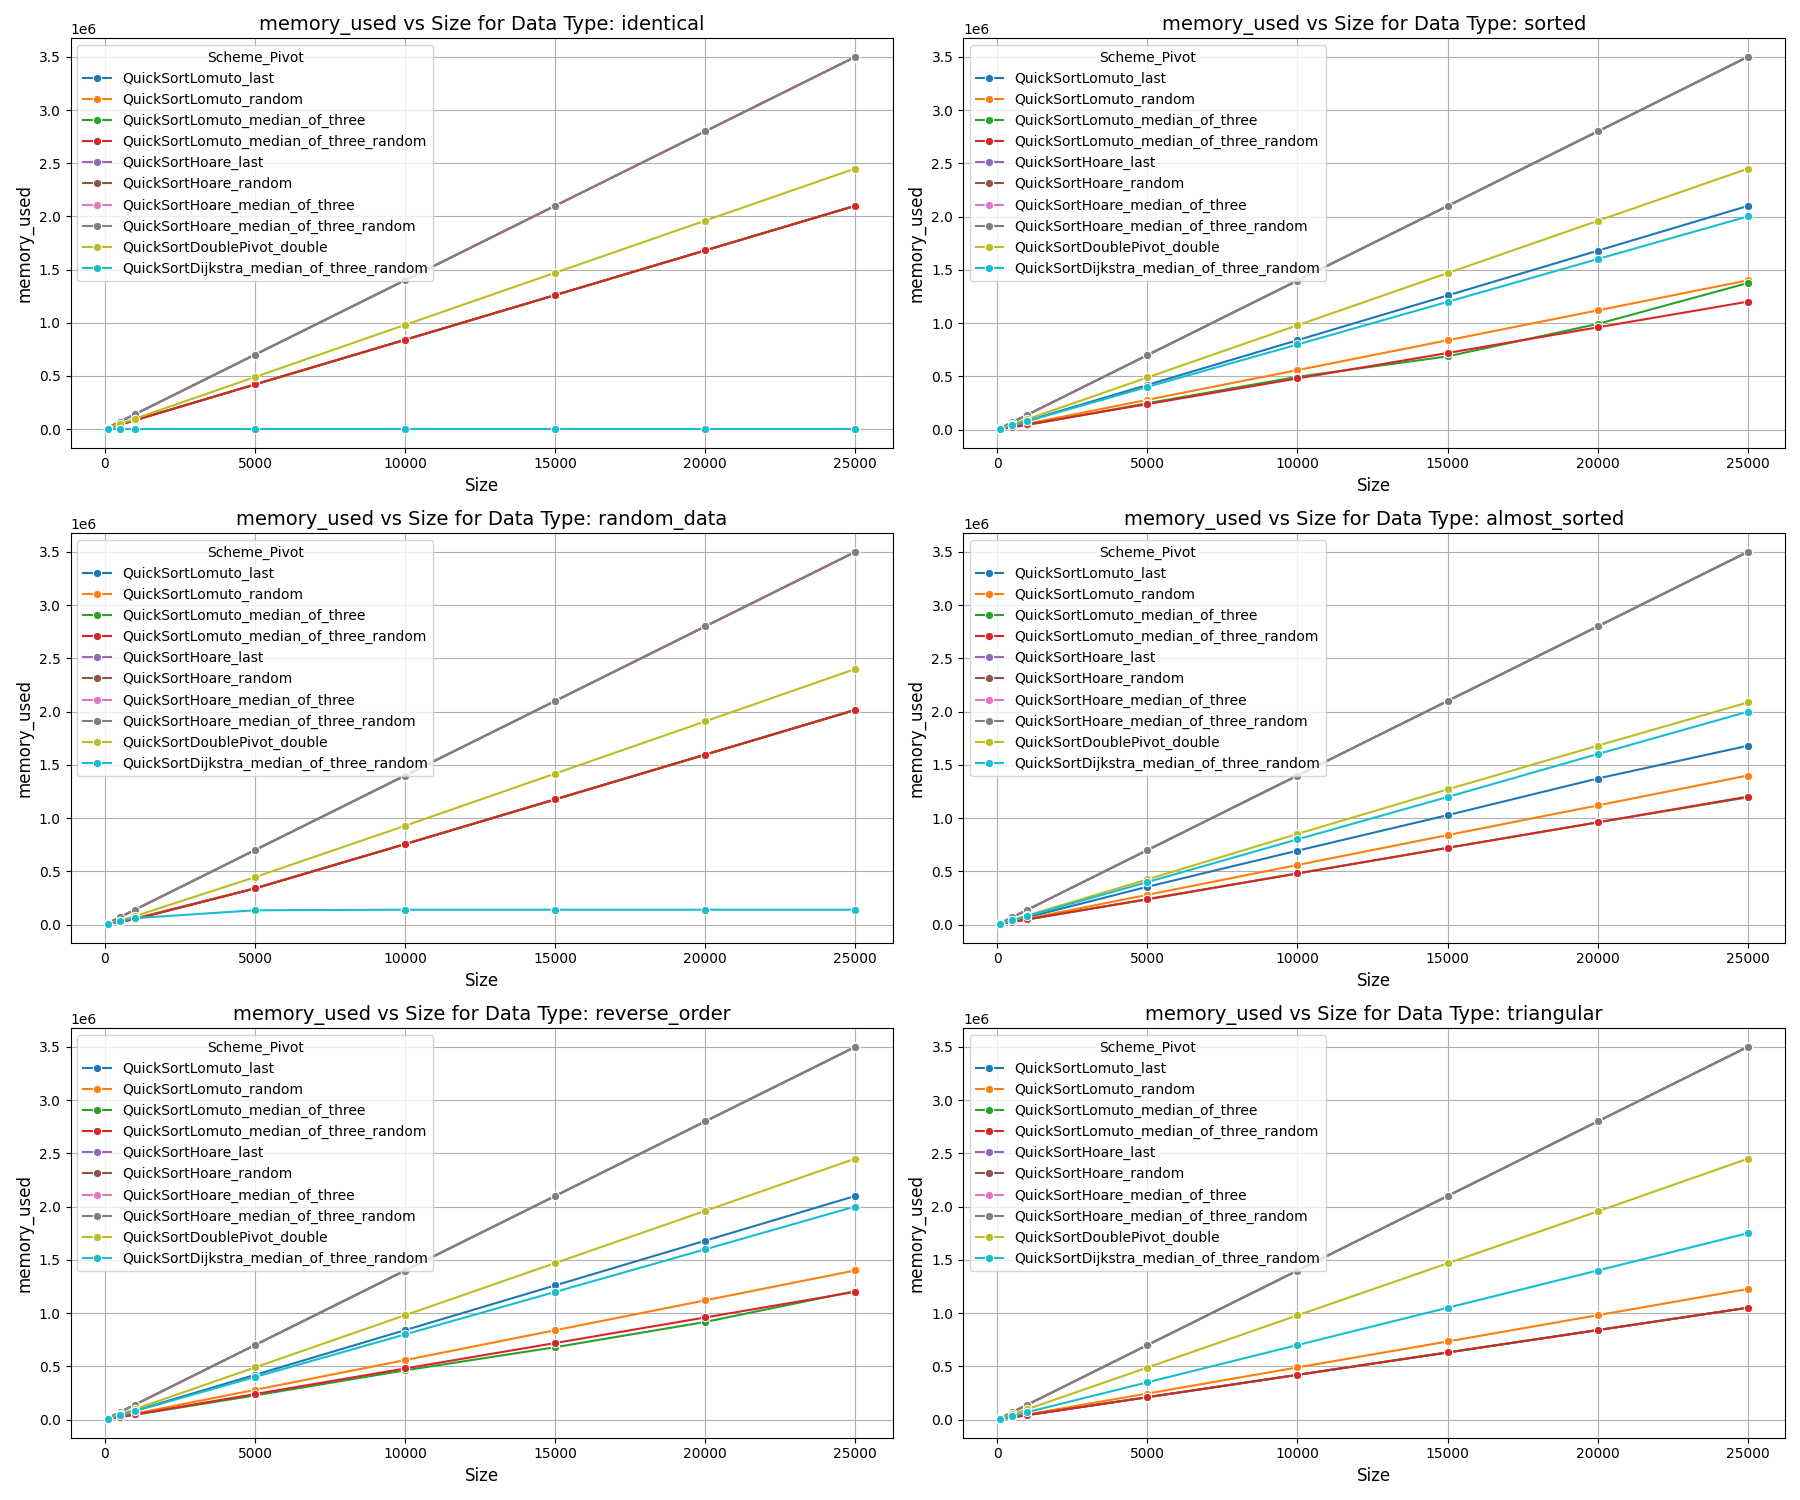
\includegraphics[width=\textwidth]{D://University/third_course/AppliedAlgorithms/lab7/memory_used_plots/memory_used_vs_size_all.png}
    \caption{Графік для використаної пам'яті (KB).}
    \label{fig:memory_chart}
\end{figure}
\newpage
\section{Найкращий алгоритм за результатами}
\begin{table}[h!]
    \centering
    \begin{tabular}{lcccc}
    \toprule
    \textbf{Data Type}      & \textbf{Time} & \textbf{Swaps} & \textbf{Comparisons} & \textbf{Memory Used} \\
    \midrule
    Identical       & Dijkstra & Dijkstra & Comparison Value & Memory Value \\
    Sorted          & Dijkstra & DoublePivot & Comparison Value & HoareMed3Rand \\
    Random Data     & Dijkstra & HoareRandom & Dijkstra & Memory Value \\
    Almost Sorted   & HoareMed3 & HoareMed3 & Dijkstra & HoareMed3Rand \\
    Memory Used     & Dijkstra & LomutoLast & Comparison Value & HoareMed3 \\
    Triangular      & Dijkstra & Swap Value & Dijkstra & HoareMed3Rand \\
    \bottomrule
    \end{tabular}
    \caption{Найкращий алгоритм для кожної категорії базуючись на графіках.}
    \label{tab:performance_metrics}
\end{table}
    
\end{document}